\documentclass{article}
\usepackage{graphicx}
\usepackage{tabularx}
\usepackage[dutch]{babel}
\begin{document}
\sffamily
\begin{titlepage}
  \centering
    \vfill
    {\bfseries\Huge
      PVA Automated Systems, \\
      Project codename Beezkneez
        \vskip2cm
      }
      {\bfseries\Large
        Mark Steijger\\
      }
      {
        \bfseries\normalsize
        0938713\\
            \vskip1cm
    }
          {\bfseries\Large
        Kazimir Piek\\
      }
      {
        \bfseries\normalsize
        0953725\\
            \vskip1cm
    }      {\bfseries\Large
        Robert Karajev\\
      }
      {
        \bfseries\normalsize
        0851997\\
            \vskip1cm
    }      {\bfseries\Large
        Michael Francis\\
      }
      {
        \bfseries\normalsize
        0963038\\
            \vskip1cm
    }
            \vskip1cm
        \today\\
    \vfill
    
\includegraphics[width=4cm]{logohr.png} % also works with logo.pdf
    \vfill
    \vfill
\end{titlepage}
\newpage
\tableofcontents

\newpage
\section{Inleiding}
Voor Tinlab Automated System wordt door 4 studenten het project codename Beezkneez uitgevoerd. Binnen dit project is het idee om door middel
van drones gedrag van bijen na te bootsen. Om dit mogelijk te maken is deze doelstelling opgesplits in 3 sub categorieen waarvoor
onderzoek en keuzeonderbouwing in dit document behandeld worden. De 3 onderdelen zijn image processing, gedrag en simulatie.

\newpage
\section{Onderzoek Resultaten}
\subsection{Onderzoek Image}
Een cruciaal onderdeel van een bij om eten op te sporen is hun zicht. Om dit te simuleren is er voor een camera gekozen die vanaf een bij, of in het geval van de simulatie een drone, de afstand naar andere objecten berekent. Er is maar een enkele camera nodig voor alle drones, zolang deze in ieder geval een overzicht heeft van elk object binnen de simulatie.\\
Uiteraard betekent dit dat er onderzoek gedaan moet worden naar de optimale camera voor deze taak. Er zijn niet veel eisen in dit geval, aangezien image processing het mogelijk maakt om de data te verwerken dat nodig is. Met dit in gedachte zijn er twee eisen aan de camera. Ten eerste moet de camera een opname in kleur maken, aangezien er een verschil wordt gemaakt tussen het eten en de bijen door middel van kleur. Daarnaast moet de camera een minimale resolutie hebben van 480x360 px. Dit is de minimale resolutie want minder dan dat zou te weinig data leveren om te verwerken, wat dan leidt tot onnauwkeurige afstanden.\\
Er zijn een aantal onderzoeken gedaan naar de ideale camera voor een project als deze. Hierin zijn vergelijkingen gemaakt tussen de GoPro, uEye en PiCam v2. Hieruit is gebleken dat de PiCam v2 de beste optie is voor een laag-budget en klein camera die aan onze eisen voldoen.\cite{picamstudies}\\
Deze camera is gekoppeld aan een Raspberry Pi. Dit maakt het mogelijk om hier direct image processing op uit te oefenen. Image processing houdt in dat afbeeldingen worden verwerkt met behulp van de digitale data van een afbeelding. Het wordt gedaan door drie redenen: digitalisatie, verbetering of restauratie en segmentatie voor machine vision.\cite{imageprocessing} In deze toepassing gaat het vooral om de laatste reden, aangezien het nodig is om bepaalde kleuren te herkennen binnen een afbeelding om daar dan een algoritme op uit te voeren. Deze algoritme zal de afstand berekenen tussen een drone en ieder ander object om deze naar de drone te sturen zodat de drone het kan verwerken. Dit gebeurt voor ieder drone, en zo heeft elke "bij" een "zicht" van alle objecten.\\
Vervolgens is het noodzakelijk om een protocol op te stellen voor het verbinden tussen de PiCam en de drones. Hier is voor bluetooth gekozen aangezien de Raspberry Pi en de drones standaard een bluetooth module hebben, wat communicatie mogelijk maakt. Ook heeft bluetooth een range van binnen de tien meter volgens de officiele Raspberry Pi handleiding, wat al meer dan genoeg is voor dit project. Er is ook geen sprake van interference of noise, gezien alle objecten een line-of-sight hebben met elkaar. Er zijn mogelijkheden besproken zoals UWB, Wi-Fi of Serial, maar al deze opties hebben niet de voordelen die bluetooth heeft.\\
Hiermee is het duidelijk dat de camera, met de bijbehorende image processing software, een kritiek component is van het gehele systeem en om bijen zo realistisch mogelijk te simuleren.\\
\newpage

\subsection{Gedarg ondezoek}
Voor het gedrag van de bijen te kunnen verwezelijken naar een software achtige structuur, is er gebruik gemaakt van
\cite{akbari_mohammadi_ziarati_2010}. In dit artikel staat een numerieke beschrijving van het gedrag van bijen.
Hierbij worden de verschillende rollen en acties die deze dieren uit kunnen voeren beschreven
en de interpetatie voor dit project hiervan zal in dit hoofdstuk beschreven worden.

\subsubsection{Werkrollen}
In het artikel worden over verschillende rollen die de bijen kunnen aannemen namelijk; werkeloos, werkend en scouting.
Een werkelozen bij kan twee acties ondernemen, gaan scouten naar eten afvankelijk van de hoeveelheid bijen die nog aanwezig zijn in de korf,
of wachten tot hij word geroepen door een werkende bij. Een scoutende bij is op zoek naar eten buiten de bijenkorf en veranderd naar een werkende bij
wanneer hij dit eten heeft gevonden en terug gaat brengen naar de bijenkorf.\\

Een werkende bij is bezig met het halen van het voedsel, maar kan hierbij ook nog keuzes maken geraleerd met hoe goed het eten is dat hij heeft gevonden.
De waarde van dit eten wordt later op terug gekomen. Voornu is het belangrijk dat wanneer er veel eten is dan kan de werkende bij 'dansen'
om werkelozen bijen mee te nemen naar het eten. Wanneer er niet veel eten meer over is dan zal de bij niet meer dansen en direct terug gaan naar de voedselbron 
in zen eentje.

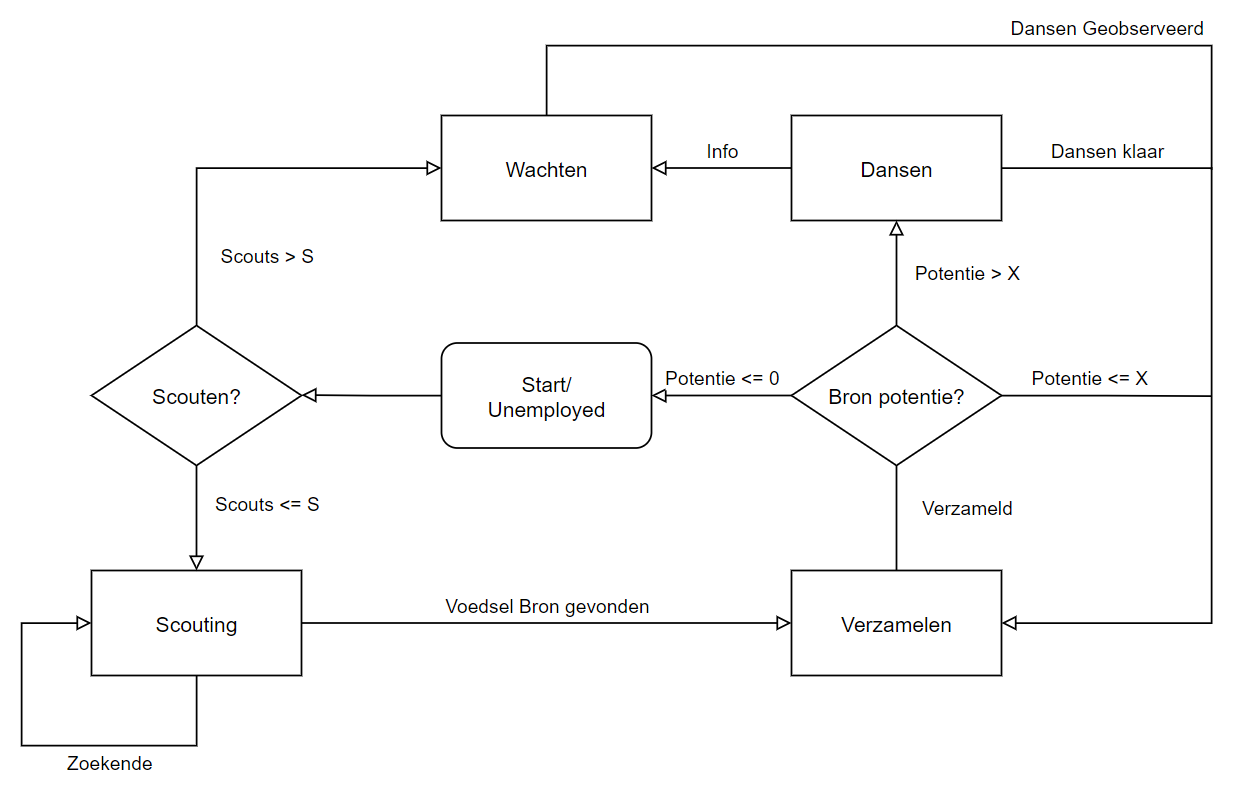
\includegraphics[scale=0.33]{../IMAGES/BijengedragFlowchart.png}

\subsubsection{Voedselpotentie}
Er zijn factoren gevormd om te bepalen hoe 'goed' het voedsel is dat gevonden is door een scout. De factoren zijn namelijk hoeveelheid voedsel die er in de bron zit 
en de afstand naar de korf toe. Door deze factoren met elkaar te vermenigvuldigen kan de potentie van een voedselbron uitgerekent worden. 
Een hogere potentie betekend dat de voedselbron 'beter' is en zou er ook voor kunnen zorgen dat meer bijen er naar toe gestuurd worden. 

\newpage
\subsection{Simulatie onderzoek}
Voor het simuleren van drones is er gekeken naar beschikbare tools waarmee dit gerealiseerd kon worden. Daarbij
zijn verschillende tools naar boven gekomen. Webots, Gazebo, V-REP en zo waren er veel meer te vinden. Daarnaast is
gekeken naar wat voor model hier het beste bij zou passen \cite{Weisberg2013}. Fysiek model wijst het beste te zijn
aangezien verplaatsing van een bij met behulp van een drone gesimuleerd moet worden. De simulatie in deze context 
zal zowel live als constructief zijn. Om dit goed te realiseren is er ook onderzoek gedaan naar wat een 
goede basis zouden kunnen vormen voor het realiseren van zulk simulatie. Daaruit is een paper over swarm simulation system
naar voren gekomen \cite{minar1996swarm}. Deze paper legt uit hoe een simulatie systeem dat in jaren 1996 gebruikt werd opgebouwt was.
Deze paper vormt dan ook een basis denkwijze voor het te realiseren simulatie systeem.

\newpage
\section{Keuze onderbouwing}
\subsection{Image gedrag}
Uit het onderzoek is gebleken dat het gedrag van de werk bijen onderverdeeld kan worden in 2 belangrijke rollen, het zoeken naar bloemen met nectar en het oogsten van de bloemen. Maar elke bij kan elke rol vullen, dus dat willen wij ook naar voren brengen in onze swarm. Aan het begin kiezen wij een willekeurige bij om als eerste eten te zoeken. Zodra deze bij het eten gearriveerd is, land hij om te bevestigen en dan keert hij terug naar de korf. Zodra hij terug bij de korf is gaat hij eerst dansen om de andere bijen te laten weten dat er in de buurt eten te vinden is. Vervolgens gaan alle beschikbare bijen in 'oogsten' mode en vliegen dus naar het eten toe om een gedeelte van de beschikbare nectar op te halen en terug naar het nest te brengen. Elke eten bron heeft een bepaalde hoeveelheid eten en de bijen zullen blijven oogsten totdat al het eten in de bron vergaard is. Zodra het eten van deze bron op is, word er opnieuw willekeurig een bij gekozen om op zoek te gaan naar eten.
De reden dat we besloten hebben om telkens maar een enkele bij op zoektocht naar eten te sturen is omdat we besloten hebben om af te wijken van het eigenlijke 'zoeken' naar eten en in plaats daarvan gewoon met de camera kijken waar het eten is en de bij direct daarnaar toe sturen met behulp van pathfinding. Dit doen we omdat, als we echt de bijen op zoektocht willen laten gaan, hebben we bepaalde extra hardware nodig dat erg duur word als we dat op meerdere fysieke bijen willen gebruiken. Om deze reden heeft het geen zin om meerdere bijen op zoektocht te laten gaan.
\subsection{Image resultaten}
\subsection{Image simulatie}
Voor het realiseren van simulatie is gekozen voor Webots programma. De keuze hiervoor is gemaakt omdat
een simulatie programma  voor deze tinlab geleert moest worden voordat het gebruikt kon worden. 
Dit is gepaard gedaan met vak Connected Systems waarbij Webots basaal behandeld werd. Ook is deze keuze
gemaakt omdat Webots ontwikkelingen in programmeertaal Python ondersteunt aangezien Python als hoofd programmeertaal
binnen dit project gebruikt wordt. Er is voor gekozen om 3 bijen te simuleren. Dit houd in dat in de simulatie programma
3 drones gesimuleerd worden die bijen gedrag zullen vertonen. De paper die in het onderzoek behandeld werdt vormt
hier ook een mooie basis aan. Elke drone in Webots zal een entiteit zijn en elke drone zal dan ook bestuurd worden
door zogenaamde controller die in Webots geprogrammeerd wordt. Verder is er een keuze gemaakt om aan elke controller
dan ook een eigen communicatie link te verbinden. De conrete protocol zal later gekozen worden.


\newpage
\bibliography{references}
\bibliographystyle{plain}
\end{document}


